\input preamble.tex
\noindent
{\bf Arbeidsoppdrag 01 - Gandsfjorden Gondol}

\vskip 5pt

Oppgaven din er å planlegge, sette i drift og dokumentere en simulert Gondolbane. Oppkoblingen skal skje på IO-Treningsbrett. Målet med arbeidsoppdraget er repitisjon, samt å gjøre dere kjent med utstyr og software vi bruker på VG3 Automasjon. 

\vskip 5pt

Typiske ny kunnskap du må lære deg er:
\begin{itemize}[noitemsep]
	\item PLS programmeringsverktøyet Codesys
	\item Koblinger på Gand PLS 01 og Gand RIO-Trainer
	\item Tegnstandard for 3AUA. 
\end{itemize}

Fokus for repitisjon
\begin{itemize}[noitemsep]
	\item Skjemategning
	\item Programmering av kominatoriske styringer
	\item Nødstopp og sikkerhetsrelaterte deler av styresystemer
	\item Asynkronmotoren
	\item Motorstartere
	\item Elektrisk utstyr i maskinger (NEK-EN 60204-1)
\end{itemize}

\vskip 5pt
Følgende tabel er en liste over oppgaver som gruppen må fullføre i den oppsatte tiden til arbeidsoppdraget. Legg merke til at noen av oppgavene har en (I), dette står for individuell og betyr at alle på gruppen må utføre den individuelt.

\vskip 5pt
\underbar{Tabell over fullførte oppgaver. }

% No blank lines allowed between lines of an \halign structure!
% I use comments (%) instead, so that TeX doesn't choke.
\begin{center}
\begin{tabular}{ | m{8cm} | m{1cm}| m{2cm} | } 
\hline
\multicolumn{3}{|c|}{Liste over oppgaver som skal utføres} \\
\hline
Oppgave	& Utført & Signatur \\ 
\hline
\hline
	Teging av nødvendige elektriskeskretser i h.h.t. regelverk og krav fra kunde. 	& & \\ 
	\hline
	Bestilling av nødvendig utstyr	&&\\
	\hline
	Lage arbeidsplan for arbeidet &&\\
	\hline
	Risikovurdere arbeidet&&\\
	\hline
	Montering av anlegget&&\\
	\hline
	Kalibrering av trykktransmitter (I)&&\\
	\hline
	IO-sjekk (I)&&\\
	\hline
	Igangkjøring av anlegget&&\\
	\hline
	Verifikasjon av anlegget (Koblinger, sikkerhet og funksjon) (I) &&\\
	\hline
	Dokumentajon av anlegget (I)&&\\
	\hline
\end{tabular}
\end{center}


\vskip 10pt
{\bf Det er viktig at din gruppe planlegger hva dere skal gjøre hver dag. Et kort morgenmøte(5min)er en god måte å gjennomføre dette på. Da kan dere gå igjennom hva dere har gjort og hva som gjenstår. Det er masse arbeid å planlegge, montere, igangsette og dokumentere et anlegg.}

\vskip 10pt
Når dere arbeider på dette anlegget kommer dere mest sansynlig borti flere problemer. Dere må alltid løse disse problemene som en gruppe før dere spør en lærer om hjelp. Om dere likevel skulle trenge hjelp av en lærer skriv gruppenummeret deres på tavelen sammen med en beskrivelse av problemet. Læreren vil hjelpe gruppene i den rekkefølgen som står på tavlen. 





\vfil \eject

\noindent
{\bf Gruppemøte, arbeidstegninger og valg av utstyr }

\vskip 5pt

%An important first step in completing this lab exercise is to {\bf meet with your instructor} as a team to discuss safety concerns, team performance, and specific roles for team members.  If you would like to emphasize exposure to certain equipment (e.g. use a particular type of control system, certain power tools), techniques (e.g. fabrication), or tasks to improve your skill set, this is the time to make requests of your team so that your learning during this project will be maximized.

\vskip 10pt

Et nødvendig steg for å fullføre dette arbeidsoppdraget, er å jobbe sammen som en gruppe om å lage arbeidstegninger for anlegget. Arbeidstegningene består som regel av arrangementstegning, skjema over elektriske koblinger og sløyfeskjema over eventuelle instrumentsløyfer. Dette trenger ikke være komplette tegninger over anlegget, men det må inneholde nok detaljer til å læreren kan avgjøre om komponentene blir rett koblet for sikker funksjon.

%For example, if you intend to connect field devices to a PLC (Programmable Logic Controller), your prototype sketch must show how those devices will connect to typical input/output terminals on the PLC, where electrical power will be supplied, etc.  Prototype sketches need not show all intermediary connections between components, such as terminal blocks in junction boxes between the field device and the controller.



%You should practice good problem-solving techniques when creating your prototype sketch, such as consulting equipment manuals for information on component functions and marking directions of electric current, voltage polarities, and identifying electrical sources/loads.  Use this task as an opportunity to strengthen your analytical skills!  Remember that you will be challenged in this program to do all of this on your own (during ``capstone'' assessments), so do not make the mistake of relying on your teammates to figure this out for you -- instead, treat this as a problem {\it you} must solve and compare your results with those of your teammates.

Gruppen sine arbeidstegninger er så viktige at læreren vil kreve at denne er klar før noe arbeid på anlegget starter. \textit{Grupper som starter arbeidet før, stoppes og får ikke starte opp før arbeidstegninger er klare.  } For at alle i gruppen skal ha tilgang på all dokumentasjon til en hver tid må gruppen jobbe i den mappen som er blitt tildelt av læreren. Å kunne lage arbeidstegninger er en viktig kompetanse som dere må trene opp på skolen og ta med dere i arbidslivet.  


\vskip 10pt


Valg av utstyr for dette arbeidsoppdraget er i stor grad gjort for dere da dere skal jobbe på IO-treningsbrettet. 

Sett dere inn i manualene for utstyret for å finne ut hvordan alt skal kobles. 


\vskip 10pt


{\bf Virkemåten til anlegget skal  være som følger:}
\vskip 10pt 

{\bf Sikkerhetsrelatere deler av styringen}
\vskip 10pt
Klar lys/knapp: For å gjøre gondolen klar for start trykkes klarkanppen og en får et klarlys(grønt) om at sikkerhetsrelatertedeler av styresystemet er ok. To endebrytere og en nødstoppknapp skal utløse sikkerhetsfunksjonen. 
\vskip 10pt 

\textbf{Vanlig styring:}
\vskip 10pt 

Normal start: Når gondol står i stopp posisjon, startes den med startknapp og går til andre siden.
\vskip 10pt 
Manuell kjøring: Når gondolen ikke går automatisk skal det være mulig å kjøre den manuelt med en vribryter. 

\vskip 10pt 
Start med gondol mellom stopposisjoner: Gondol kjøres manuelt i ønsketstartretning, samtidig holdes startknappen inne i 5sek, nå skal Gondolen gå over i automatisk kjøring mot stopposisjon.
\vskip 10pt 
Alarm: Trinsene som Gondolen kjører på har et glidelager. Ved lavt trykk her skal det gis alarm. Lavt trykk er definert som 0.7 bar. Trykkmåleren som brukes skal ha et måleområde på 0-2 bar. Alarmsignalet skal få et lys til å blinke. Når en trykker på en bekreft knapp skal lyset gå over til å lyse konstant. (Det vil normålt også være et lydsignal til en alarm, dette brukes ikke i dette arbeidsoppdraget). Alarmen resettes automatisk når trykket overstiger 0.9 bar. 
\vskip 10pt 
{\bf Planlegging av anlegget bør ikke ta mer en to timer med effektivt arbeid. }
\vfil \eject

\noindent
{\bf Bygging av maksinen}

\vskip 5pt

IO-treningsbrettet er lagt opp for å etterligne en vanlig installasjon i en maskin. Styreskapet er simulert og har en vegg der kabler kommer ut i nipler. Kablene skal så gå på en kabelgate før de kommer frem til utstyret. Alt skal gjøres mest mulig virklighetstro. Ledere som skal ut av styreskapet skal igjennom rekkeklemmer og via kabler på kabelstige ut til utstyret. Ledere som skal døren på styreskapet skal i en spiral. 


$$\includegraphics[width=15.5cm]{arb01x01.eps}$$
$$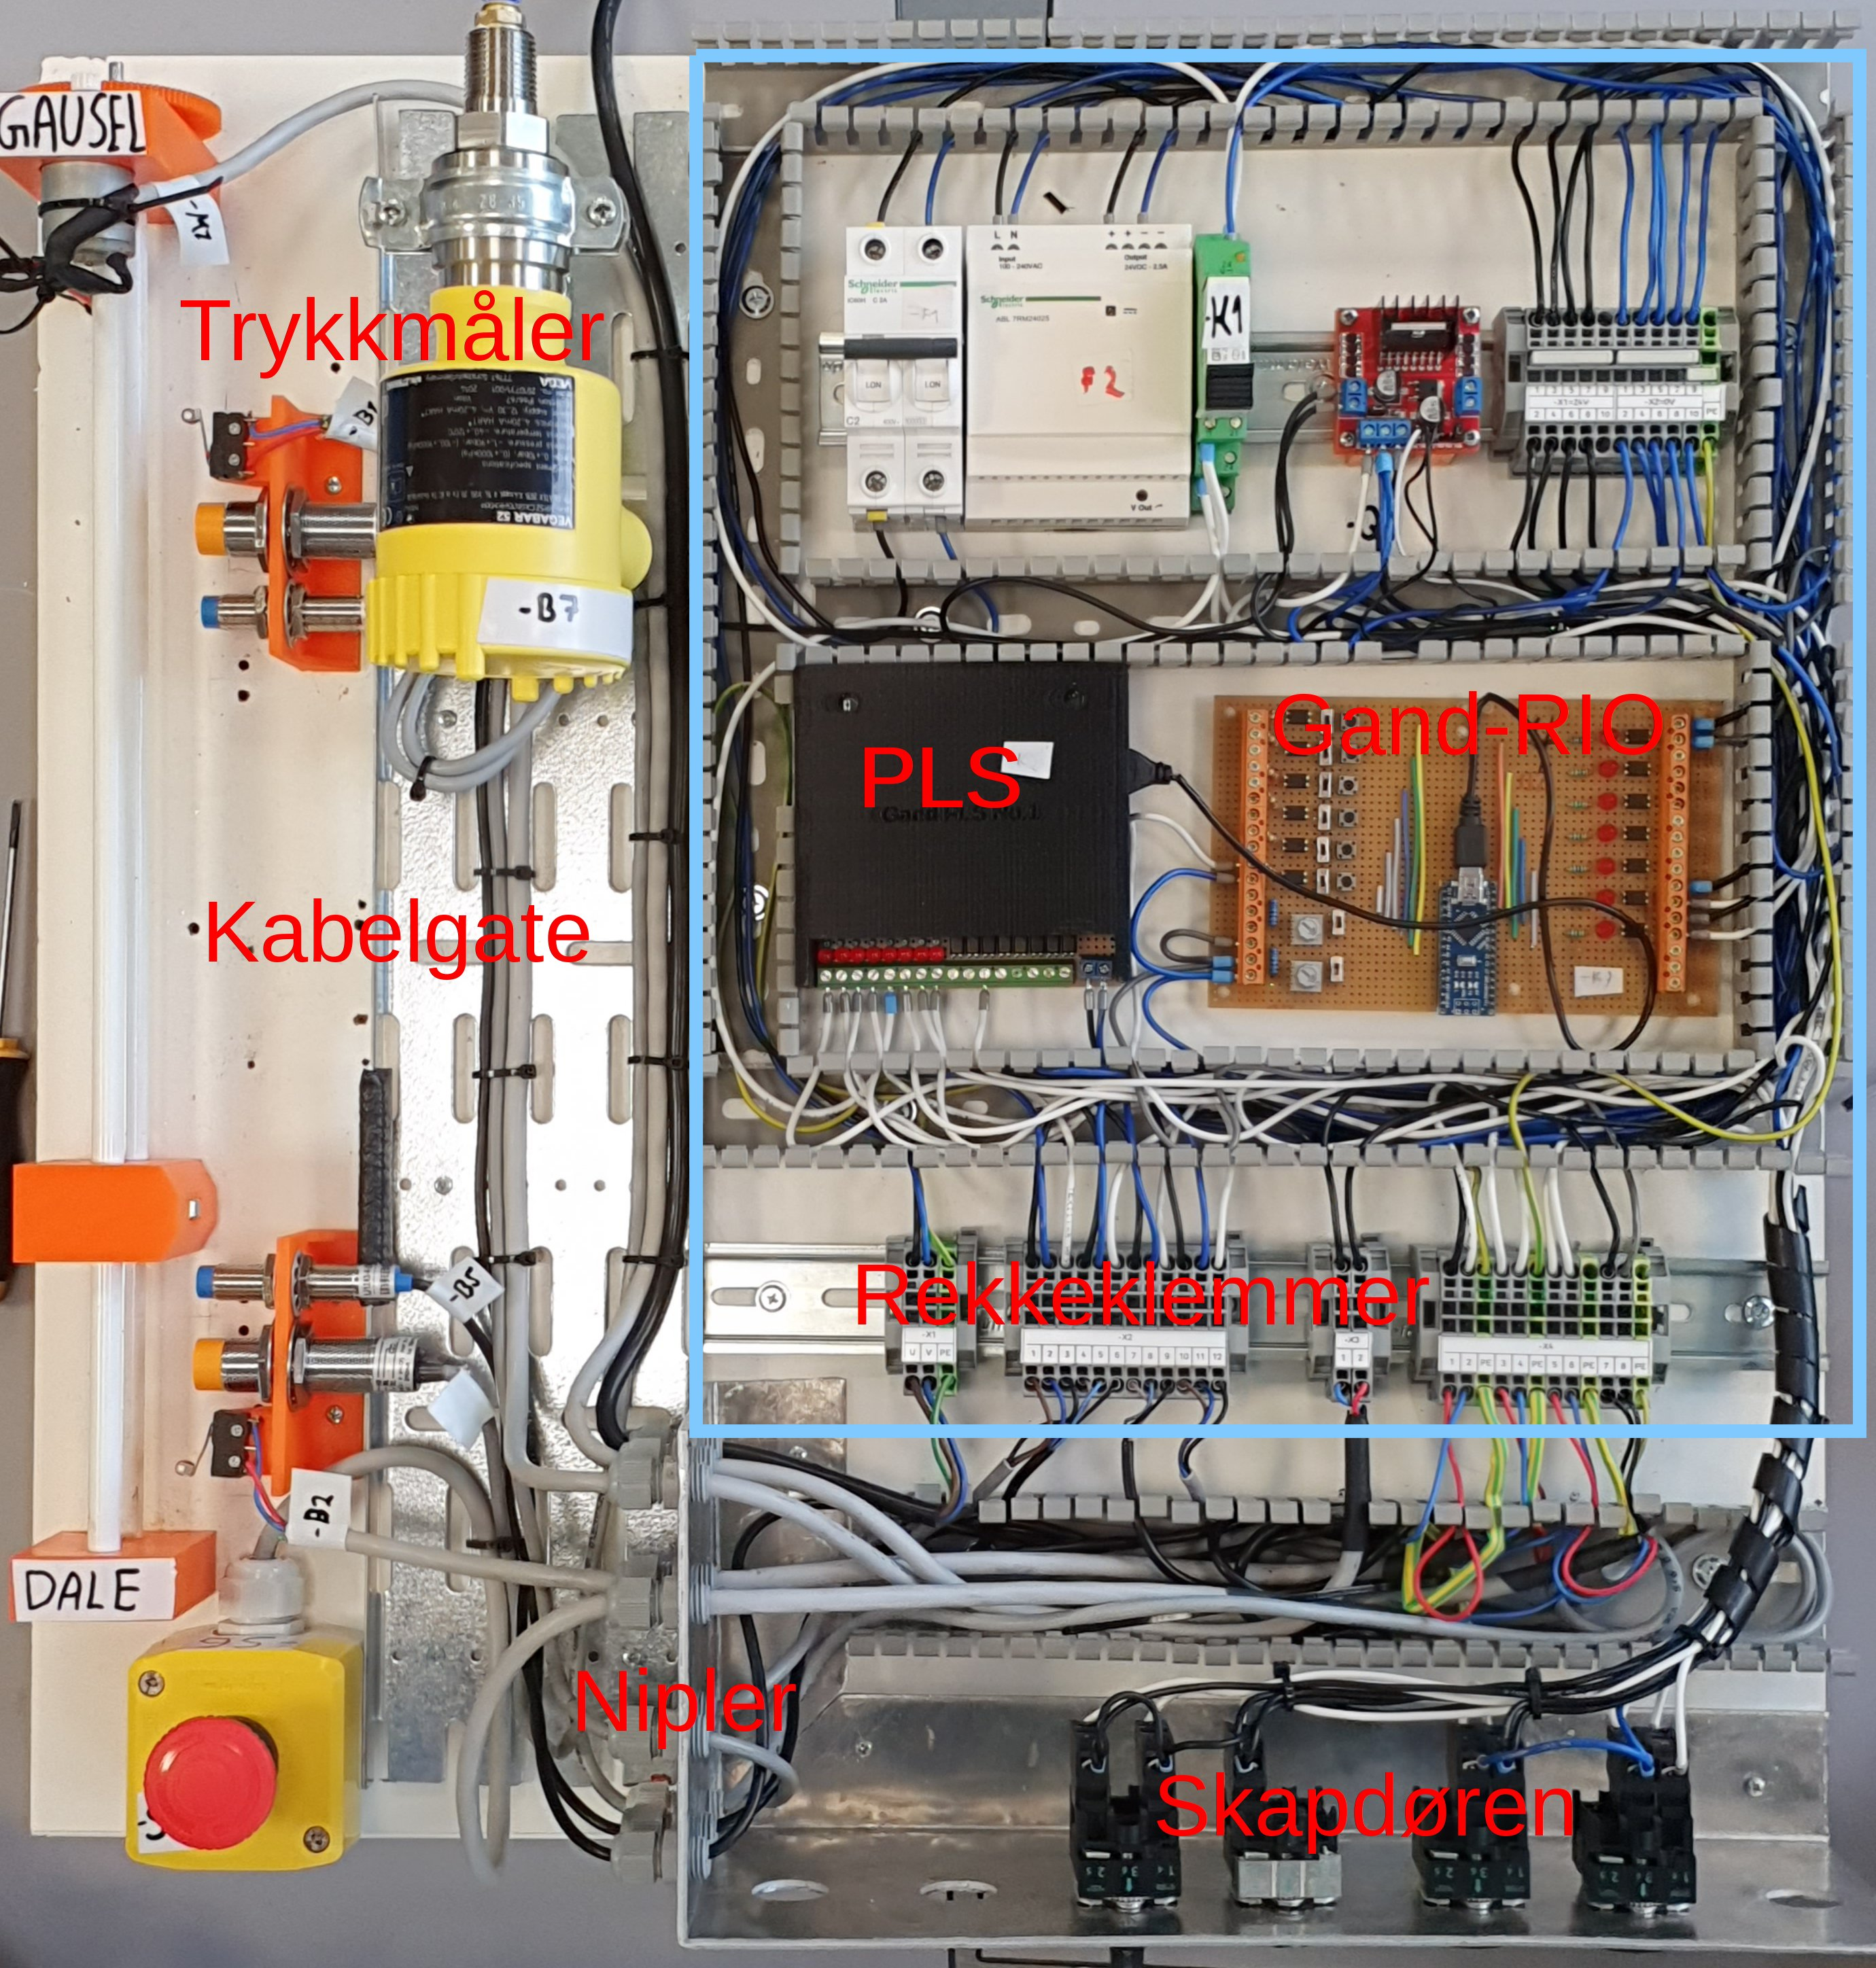
\includegraphics[width=15.5cm]{arb01x02.jpg}$$
Når gruppen har fått godkjent arbeidstegningene. Kan dere starte byggingen av maskinen.  


\vskip 10pt

\textbf{Vanlige Feil}
\begin{itemize}[noitemsep]
	\item Ikke sjekke utstyrmanualer fra produsenter, om hvordan des settes opp og kobles. 
	\item Ikke feste ledere passe hardt, fører enten til enten løse ledere eller ødelagte tilkoblingsterminaler.
	\item Elever arbeider på en del av systemet for seg selv. Det er viktig at alle i gruppen kan hele systemet og kan svare på spørsmål om det.  
\end{itemize}

\vskip 10pt 

\textbf{Byggingen av maskinen bør ikke ta med en 15timer (en uke)}

\vfil \eject

\noindent
\textbf{Dokumentajon av anlegget}

\vskip 10pt 
Dokumentasjonen skal bestå av:
\begin{itemize}[noitemsep]
	\item Beregninger (beregninger av kabler og ledere)
	\item Tegninger (Komplett elektrisk skjema, arrangementstegning av brett sett oppenifra og sett rett på bryterpanel, grafisk kabelplan og rekkeklemmeliste.)
	\item Skjema for verifikasjon av elektrisk utstyr i en maskin
	\item Alle merkefiler
	\item PLS program
	\item Kalibreringssertifikat
	\item Manualer for alt utstyr
	\item Bilder fra anlegget
	\item Logg
\end{itemize}


Hver elev må lage sin versjon av dokumentasjonen ut fra utskrevet skjema fra forberedelsen. 





\vskip 10pt

\textbf{Vanlige Feil}
\vskip 10pt
\begin{itemize}[noitemsep]
	\item Ikke merke alle komponenter og ledninger
	\item Ikke følge mal for dokumentajson i 3AUA
\end{itemize}


\vskip 10pt






\vfil \eject

\noindent
\textbf{Kalibrering av trykktransmitter}

\vskip 5pt

IO-brettet inneholder en trykktransmitter som må settes opp og kalibreres før bruk. Oppsett og kalibreringsresultater føres på kalibreringsmal for 3AUA. Det skal utføres 5-punkts kalibrering opp og ned. 



\filbreak


\vskip 10pt


\vskip 10pt

\textbf{Vanlige feil:}
\begin{itemize}[noitemsep]
	\item Ingen foreløbig
\end{itemize}


\vskip 10pt

\textbf{Klargjøring av transmitteren bør ikke ta mer tid en 1 time}




\vfil \eject



\underbar{file arb01}





















\vfil \eject

\noindent

\vskip 20pt
\end{document}

